\section{Using a Black Hole Starship}
	Up until now, the modes of transport have at least been somewhat realistic.
	Now, we enter the area of theoretical transportation. The details of how a black hole starship functions are outside the scope of this paper (and would add roughly 20 more pages), so we will only cover the basics.
	
	In order for a black hole starship to function, a very small black hole must be created.
	Specifically, the Schwarzschild radius of the black hole (distance from the centre at which light cannot escape the gravitational force) should be about \SI{9e-19}{\metre} \autocite{blackHoleStarship}.
	This small black hole will be placed at the focal point of a parabolic reflector, which is attached to the starship \autocite{blackHoleStarship}.
	The black hole will emit a type of energy called Hawking radiation which reflects off the parabolic reflector and propels the ship forward with immense energy.
	According to \cite{blackHoleStarship}, a proposed system with a black hole of mass \SI{6.06e8}{\kg} should be able to accelerate to \SI{0.1}{\clight} in 20 days. 
	\begin{figure}[H]
	\caption{Diagram of a black hole starship. The Hawking radiation from the black hole reflects and propels the starship.}
	\label{fig:blackHoleStarship}
	\centering
	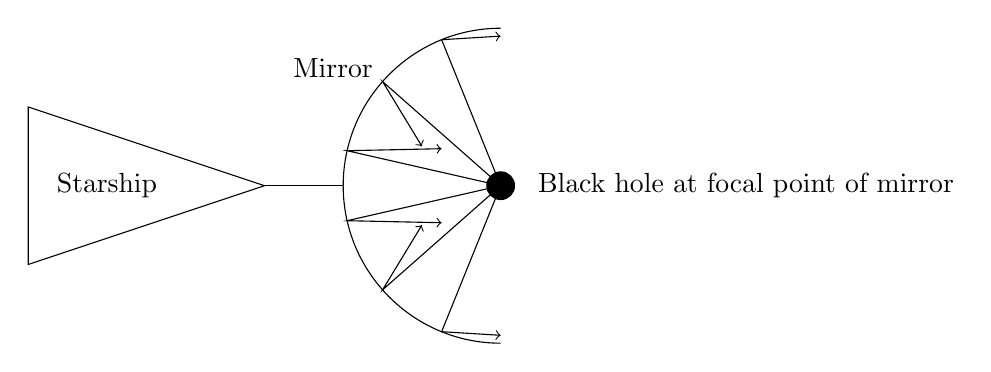
\begin{tikzpicture}
		\coordinate [label=center:Starship] (ShipCentre) at (-2,0);
		\coordinate (ShipTip) at (0,0);
		\coordinate (ShipTopLeft) at (-3,1);
		\coordinate (ShipBottomLeft) at (-3,-1);
		\coordinate [label={[label distance=1em] right:Black hole at focal point of mirror}] (BlackHole) at (3,0);
		\coordinate [label=above left:Mirror] (Mirror) at (1.5,1.25);

		\draw (ShipTopLeft) -- (ShipTip) -- (ShipBottomLeft) -- cycle;

		\draw (3,2) arc (90:270:2);

		\draw (ShipTip) -- (1,0);

		\draw [->] (BlackHole) -- (2.25,1.854049622) -- (3,1.9);
		\draw [->] (BlackHole) -- (2.25,-1.854049622) -- (3,-1.9);

		\draw [->] (BlackHole) -- (1.5,1.322875656) -- (2,0.5);
		\draw [->] (BlackHole) -- (1.5,-1.322875656) -- (2,-0.5);

		\draw [->] (BlackHole) -- (1.05,0.4444097209) -- (2.25,0.47);
		\draw [->] (BlackHole) -- (1.05,-0.4444097209) -- (2.25,-0.47);

		\filldraw[black] (BlackHole) circle (5pt);
	\end{tikzpicture}
\end{figure}

	As with the space shuttle, we will be calculating acceleration since the black hole starship will be travelling in space.
	In addition, since the top speed is reasonably close to the speed of light, we must account for time dilation and cannot simply use the kinematics formula for acceleration.
	Recall from \cite{sracceleration} that:
	\[v = \si{\clight} \tanh \left(\frac{aT}{\si{\clight}}\right)\]
	This can be rearranged to solve for acceleration:
	\begin{align*}
		a &= \frac{\si{\clight} \arctanh \left(\frac{v}{\si{\clight}}\right)}{T}\\
		a &= \frac{\SI{299792458}{\metre/\second} \times \arctanh \left(\frac{0.1(\SI{299792458}{\metre/\second})}{\SI{299792458}{\metre/\second}}\right)}{20 \times 24 \times 60 \times 60}\\
		a &\doteq \SI{17.407}{\metre/\second^2}
	\end{align*}
